% źródła: 
% Tadeusiewicz - Sieci Neuronowe
% http://www.cogsys.wiai.uni-bamberg.de/teaching/ws1112/km/practice/ANNs.pdf
% brief introduction to neural networks david kriesel
% http://neuralnetworksanddeeplearning.com

% default activate function: TanSig 
% default tarin function -> Gradient descent with momentum backpropagation and adaptive lr, hiperbolic tangent
\section{Sztuczne sieci neuronowe}\label{rozdzial_sieci}
Sztuczną siecią neuronową, dalej zwaną po prostu siecią neuronową, określamy model matematyczny służący jako system przetwarzania informacji. Źródłem inspiracji dla tegoż modelu była biologia, a~mianowicie sieci neuronowe istniejące w~ludzkim mózgu. Dużą zaletą sieci neuronowych jest fakt, iż nie działają jak tradycyjne algorytmy, lecz mają one zdolność do uczenia się. Jest to kolejna analogia związana z pracą ludzkiego mózgu, co powodowało wzrastające zainteresowanie tym tematem. Pomimo tego, że nie udało się z ich pomocą odtworzyć pracy tego niewątpliwie niesamowitego narządu, znajdują one zastosowanie w wielu dziedzinach nauki. Najbardziej podstawowym rodzajem sieci neuronowej jest sieć jednokierunkowa tj. czyli taka, w której nie występują sprzężenia zwrotne i~takie też sieci są wykorzystane w~tej pracy oraz opisane w~tym rozdziale.

%„Neuron McCullocha-Pittsa” autorstwa Wersję rastrową wykonał użytkownik polskiego projektu wikipedii: Andrut, Zwektoryzował: Krzysztof Zajączkowski - Wersja rastrowa: http://pl.wikipedia.org/wiki/Plik:Neuron_McCullocha-Pittsa.png. Licencja CC BY-SA 2.5 na podstawie Wikimedia Commons - https://commons.wikimedia.org/wiki/File:Neuron_McCullocha-Pittsa.svg#/media/File:Neuron_McCullocha-Pittsa.svg
%
\subsection{Budowa sieci neuronowej}
Szczegółowy opis zagadnień związanych z budową sieci neuronowej można znaleźć w pracy \cite{tadeusiewicz}.
\subsubsection{Budowa neuronu}
Sieć neuronowa zbudowana jest z~neuronów, które są odpowiednikami komórek nerwowych. Synapsy łączące poszczególne komórki modelowane są przez wagi liczbowe, których wielkości z kolei można interpretować jako wpływ jednej komórki na drugą. Matematyczny model neuronu użyty w sieciach neuronowych jest przedstawiony na rysunku \ref{neuron}. Składa się on z~$n+1$ wejść oraz jednego wyjścia. Dodatkowym wejściem neuronu jest tzw. bias, który przyjmuje stałą wartość, ale jest także modyfikowany w procesie uczenia (podobnie jak pozostałe wagi). Najczęściej przyjmuje się, że przed rozpoczęciem uczenia jego wartość równa jest $1$. Zależność pomiędzy sygnałami wejściowymi $x_i$, wagami $w_i$, a~tzw. sygnałem sumarycznego pobudzenia $\varphi$, w najprostszym przypadku może być określana przez wzór:
\begin{equation}
\varphi=w_0 + \sum_{i=1}^{n}w_i x_i.
\end{equation}
Sposób obliczenia sygnału wyjściowego neuronu określany jest przez funkcję aktywacji:
\begin{equation}
y=f(\varphi).
\end{equation}
Powszechnie używa się czterech funkcji aktywacji: funkcji liniowej, funkcji sigmoidalnej, funkcji tangens hiperboliczny oraz funkcji Gaussa\cite{leksykon}. Wzory poszczególnych funkcji znajdują się w~tabeli \ref{table:activation}, natomiast na rysunku \ref{funkcje} przedstawione zostały ich wykresy.

\begin{table}
\centering
\begin{tabular}{|c|c|}
\hline
funkcja & wzór \\
 \hline
liniowa  & $y=x$ \\  
 \hline
sigmoidalna  & $y=\frac{1}{1+e^{-x}}$ \\  
 \hline  
tangensoidalna  & $y = \frac{1-e^{-2x}}{1+e^{-2x}}$ \\  
\hline 
Gaussa & $e^{-x^2}$\\  
\hline 
 \end{tabular}
 \caption{Funkcje aktywacji wraz z ich wzorami} \label{table:activation}
\end{table}

\begin{figure}[ht!]
\centering
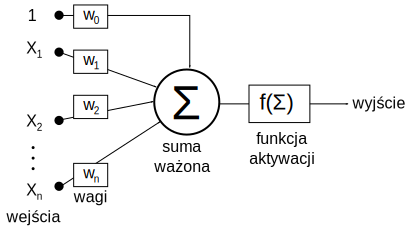
\includegraphics{res/neuron.png}
\caption[Caption for LOF]{Matematyczny model neuronu\label{neuron}\footnotemark}
% \caption{Matematyczny model neuronu\label{neuron} Źródło:\footnote{aa} } 
\end{figure} 


%obrazek z leksykonu
\begin{figure}[ht!]
\centering
\includegraphics[scale=0.45]{res/funkcje.png}
\caption{Najczęściej używane funkcje aktywacji\cite{leksykon}\label{funkcje}}
\end{figure} 

\subsubsection{Topologia sieci}
\footnotetext{\url{http://pl.wikipedia.org/wiki/Plik:
Neuron_McCullocha-Pittsa.png}}
\begin{minipage}[adjusting]{\textwidth}
Wszystkie neurony zgrupowane są w warstwy z których możemy wyróżnić:
\begin{itemize}
\item warstwę wejściową
\item jedną lub więcej warstw ukrytych
\item warstwę wyjściową
\end{itemize}
\end{minipage}\vspace{1cm}
W~każdej z~warstw znajduje się dowolna liczba neuronów, który posiada połączenie do wszystkich neuronów znajdujących się w~warstwie kolejnej. Przykład sieci neuronowej składającej się z~dokładnie trzech warstw zawierającej różną ilość neuronów w każdej z~nich został przedstawiony na rysunku \ref{net}.

\begin{figure}[ht!]
\centering
% obrazek pobrany z 
\includegraphics{res/exampleNet.png}
\caption[Caption for LOF]{Przykładowa jednokierunkowa sieć neuronowa\label{net}\footnotemark} 
\end{figure}
\footnotetext{\url{https://2ml4pa.bn1303.livefilestore.com/y2p6no6Dn0weHW3FG9tceTUS9lohx5ldcxvFZRhKdbeFQi2kntad_77gKeKIC-INcsFRCvGI-_DY9lMdZzaX8jkSHDvqlcT3qRnftpAt7esi4s/1.PNG?psid=1}}
%Źródło:\url{https://2ml4pa.bn1303.livefilestore.com/y2p6no6Dn0weHW3FG9tceTUS9lohx5ldcxvFZRhKdbeFQi2kntad_77gKeKIC-INcsFRCvGI-_DY9lMdZzaX8jkSHDvqlcT3qRnftpAt7esi4s/1.PNG?psid=1}}

\subsection{Uczenie sieci neuronowej} 
Wyróżniamy dwa podstawowe sposoby uczenia sieci:
\begin{itemize}
\item uczenie z nauczycielem (uczenie nadzorowane) - gdy dysponujemy danym treningowymi
\item uczenie bez nauczyciela (uczenie nienadzorowane) - gdy nie dysponujemy danymi treningowymi, a~sieć neuronowa klasyfikuje dane znajdując podobieństwa pomiędzy przypadkami 
\end{itemize}
W~niniejszej pracy zastosowane zostało uczenie sieci z~nauczycielem. Dzięki możliwości uczenia sieci neuronowej nie jest konieczne projektowanie algorytmu, który przetwarza dla nas informacje w oczekiwany sposób. Sieć neuronowa korzystając z~odpowiedniego algorytmu uczenia sama modeluje ten algorytm poprzez modyfikację wag. Należy też wspomnieć, że początkowe wagi sieci neuronowej zwykle inicjalizowane są wartościami losowymi.   

\subsubsection{Reguła delta}
Proces uczenia polega na modyfikowaniu współczynników wagowych sieci neuronowej. Opisane w tym podrozdziale zostanie uczenie z~nauczycielem, ponieważ takie właśnie zostało wykorzystane w~tej pracy. W~przypadku uczenia z~nauczycielem potrzebujmy zbioru uczącego składającego się z~wektora danych, które podajemy na wejście sieci i~oczekiwanego rezultatu dla tego przypadku, co możemy oznaczyć jako pary $(y_i,z_i)$, gdzie $z_i$ jest oczekiwaną odpowiedzią dla sygnału wejściowego $x_i$. Zadaniem sieci jest modelowanie funkcji:
\begin{equation}
h(x)=z.
\end{equation}
Uczenie jest procesem iteracyjnym, gdzie w~każdej iteracji modyfikujemy wagi sieci. Liczba iteracji $N$ równa jest liczbie par $(x_i,z_i)$. W~każdym kroku $j$ procesu uczenia możemy zdefiniować wielkość błędu neuronu wyjściowego jako:
\begin{equation}
\delta_i^j = |z_i^j - y_i^j|,
\end{equation}
gdzie $y_i$ jest odpowiedzią sieci neuronowej dla sygnału $x_i$.
Proces uczenia jest realizowany poprzez minimalizację funkcji:
\begin{equation}\label{minFunc}
Q=\frac{1}{2}\sum_{j=1}^{N}(\delta_i)^2
\end{equation}
będącej miarą dopasowania funkcji metodą najmniejszych kwadratów. Korzystając z metody gradientowej możemy zdefiniować poprawkę $\Delta w$ dla wagi $w$ neuronu $i$ jako:
\begin{equation}\label{deltaRule}
\Delta w_i = - \eta \frac{\partial Q}{\partial w_i},
\end{equation}
oraz, idąc dalej, zdefiniować wzór korygujący wagi $w$ w kolejnych krokach:
\begin{equation}
w^{j+1}_i = w^j_i + \Delta w_i
\end{equation}
przy czym $\eta$ jest dodatkowym współczynnikiem liczbowym, który decyduje o szybkości uczenia. W ten sposób poprawiamy wagi sieci $j$ razy. Problemem z~którym borykano się do połowy lat 80-tych jest fakt, iż tym sposobem niemożliwe jest uczenie sieci, która składa się z~więcej niż jednej warstwy, ponieważ nieznana jest oczekiwana odpowiedź neuronów warstwy innej niż wyjściowej. Wzór \ref{deltaRule} jest jednak podstawą większości algorytmów automatycznego uczenia\cite{tadeusiewicz} i~jest on określany w literaturze regułą delta\cite{briefIntroduction}.

\subsubsection{Algorytm wstecznej propagacji błędów}
W~celu przeprowadzenia uczenia dla sieci wielowarstwowej spotykamy się z~potrzebą określenia błędu $\delta$ dla neuronów, które należą do warstw ukrytych sieci neuronowej. Umożliwia nam to algorytm wstecznej propagacji błędów. Błąd dla takiego neuronu obliczamy korzystając ze wszystkich błędów neuronów do których wysłał on swój sygnał. Uwzględniane są także wagi połączeń. Mowa jest o wstecznej propagacji, ponieważ odbywa się ona przeciwnie do przepływów sygnałów w~sieci. Błąd dla neuronów znajdujących się w~warstwie innej niż wejściowa możemy określić jako:
\begin{equation}
\delta_i = f'(\varphi) \sum_{i}^{N}w_k \delta _k,
\end{equation}
przy czym $w_k$ oraz $\delta _k$ są kolejno wagami oraz błędami neuronów do których analizowany neuron wysyłał swój sygnał.
%Korzystając z definicji pochodnej złożonej - biorąc pod uwagę, że $Q$ zależy od $y$, a $y$ od $w$ - możemy %zapisać wzór \ref{deltaRule} jako:
%\begin{equation}
%\Delta w = - \eta \frac{\partial Q}{\partial y} \frac{\partial y}{\partial w}
%\end{equation}
%biorąc pod uwagę:
%\begin{equation}
%frac{\partial Q}{\partial y} = - \delta
%end{equation}